\section{Introduction}

\begin{definition}[\textit{Dependability}]
    Dependability is a measure of the trust we place in a system.
\end{definition}
Dependability also encompasses the system's ability to perform its intended functions, characterized by the following attributes:
\begin{itemize}
    \item \textit{Reliability}: the continuous delivery of correct service.
    \item \textit{Availability}: the readiness for correct service.
    \item \textit{Maintainability}: the ease with which maintenance can be performed.
    \item \textit{Safety}: the prevention of catastrophic consequences.
    \item \textit{Security}: the protection of data confidentiality and integrity.
\end{itemize}

Substantial efforts are often devoted to functional verification to ensure the system's implementation meets specifications, fulfills requirements, adheres to constraints, and optimizes selected parameters. 
Despite addressing these aspects, system failures can still occur, usually due to some form of breakdown.
\begin{figure}[H]
    \centering
    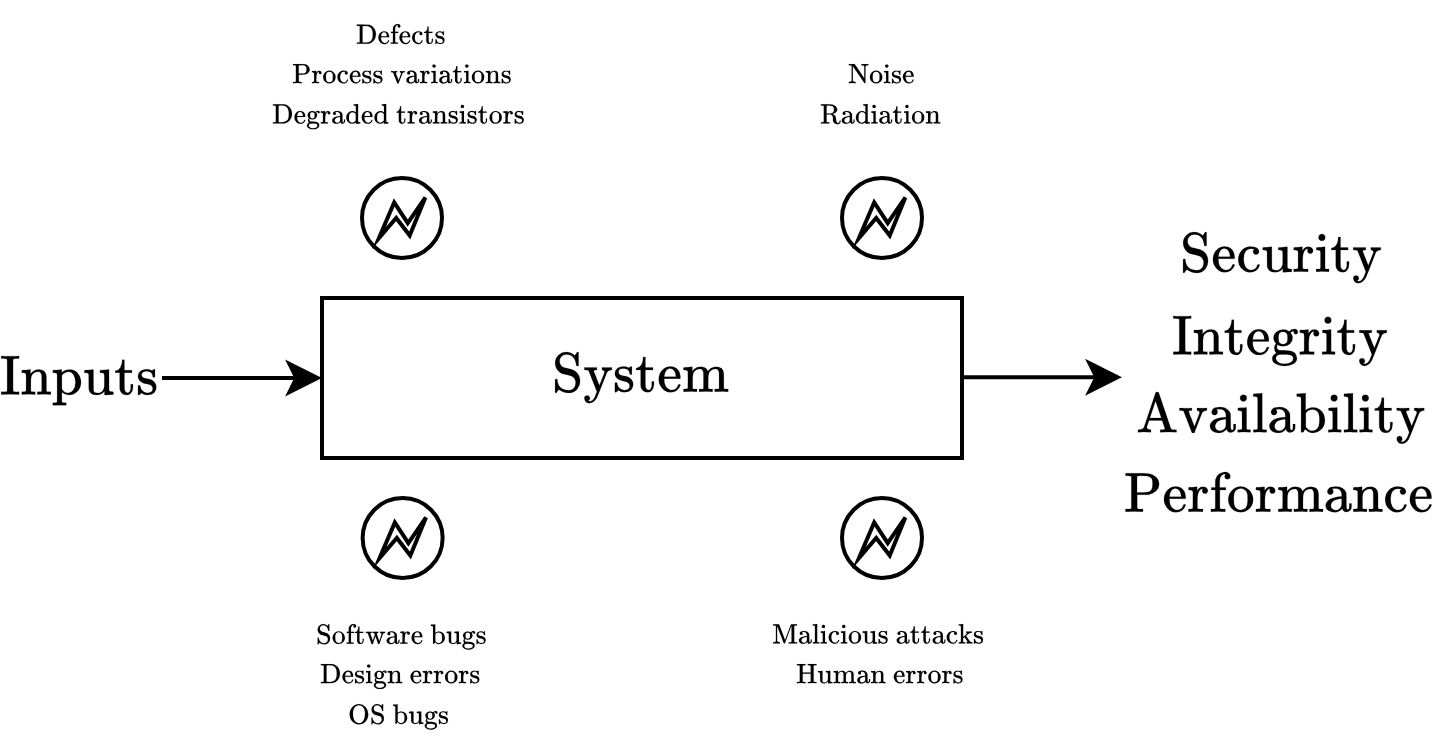
\includegraphics[width=0.75\linewidth]{images/dep.png}
    \caption{Dependability}
\end{figure}
A single system failure can impact a large number of individuals and lead to significant costs, particularly in terms of economic loss or physical damage. 
Systems that lack dependability are less likely to be adopted or trusted. 
Additionally, undependable systems can result in information loss, leading to substantial recovery expenses.